\subsection{Schema Indexing}

To choose the most relevant subset of samples from $\mathcal{S}$ for $k$-shot learning,
it is important that the SQL queries we supply are written for structurally similar SQL schemas
in order to minimize the structural difference between the supplied samples $\mathcal{S}_k$ and
the ground truth query $\omega_{ground}$ for a given natural language question.

For example $\omega_{ground}$ the question ``Give me all contacts for the user with the id 10''
might look different depending on the database schema at hand, thus only selecting
samples based on the similarity of the natural language question will yield inferior
sample quality.

\begin{figure}[ht]
  \vspace{1em}
  \hfill
  \begin{minipage}[b]{0.45\linewidth}
    \begin{verbatim}
CREATE TABLE users (
  id TEXT PRIMARY KEY
);

CREATE TABLE contacts (
  user_id TEXT NOT NULL,
  name TEXT NOT NULL,
  FOREIGN KEY (user_id) ON users(id),
  PRIMARY KEY (user_id, name)
);
    \end{verbatim}
    \caption{Normalized schema}
    \label{figure:schema-normalized}
  \end{minipage}
  \hfill
  \begin{minipage}[b]{0.35\linewidth}
    \begin{verbatim}
CREATE TABLE users (
  id TEXT PRIMARY KEY,
  contacts TEXT[] NOT NULL
);
    \end{verbatim}
    \vspace{3.75em}
    \caption{Denormalized schema}
    \label{figure:schema-denormalized}
  \end{minipage}
  \hfill
  \vspace{1em}
\end{figure}

Given the database schemas in figures~\ref{figure:schema-normalized} and~\ref{figure:schema-denormalized}
respective definitions of $\omega_{ground}$ would be:

\begin{figure}[ht]
  \vspace{1em}
  \hfill
  \begin{minipage}[b]{0.45\linewidth}
    \begin{verbatim}
SELECT contacts.name
FROM users
JOIN contacts
  ON contacts.user_id = users.id
WHERE users.id = 10;
    \end{verbatim}
    \caption{SQL JOIN selection}
    \label{figure:sql-join-example}
  \end{minipage}
  \hfill
  \begin{minipage}[b]{0.35\linewidth}
    \centering
    \begin{verbatim}
SELECT contacts
FROM users
WHERE id = 10;
    \end{verbatim}
    \vspace{1.3em}
    \caption{SQL Array selection}
    \label{figure:sql-array-example}
  \end{minipage}
  \hfill
  \vspace{1em}
\end{figure}


As shown in the figures~\ref{figure:sql-join-example} and~\ref{figure:sql-array-example}
the structural similarity of the underlying database schema is a crucial component
of the relevance of a example.

\subsubsection{Graph Representation}

In order to determine structural similarity of database schemas we propose using
graph representation of database schemas as a data definition language (DDL)
independent representation of the databases structure. Furthermore choosing a graph
representation allows us to use prevalent methods for measuring graph similarity
(eg, \textcolor{red}{Weisfeiler-Lehman graph kernels, cite}).

We define the structural similarity of two databases as the toplogical distance
of the respective \textsc{Natural}-graphs. The \textsc{Natural}-graph representation
only models tables, columns, relationships, datatypes and constraints, omitting 
table names, column names and domain terminology.

\begin{figure}[ht]
  \vspace{1em}
  \hfill
  \begin{minipage}[b]{0.45\linewidth}
    \centering
    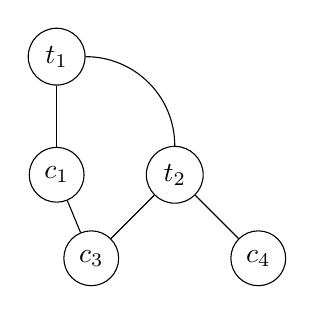
\begin{tikzpicture}[node distance={15mm}, main/.style = {draw, circle}] 
      \node[main] (1) {$t_1$}; 
      \node[main] (2) [below of=1] {$c_1$}; 
      \node[main] (3) [right of=2] {$t_2$}; 
      \node[main] (4) [below left of=3] {$c_3$}; 
      \node[main] (5) [below right of=3] {$c_4$}; 

      \draw (1) -- (2); 
      \draw (2) -- (4); 
      \draw (3) -- (4); 
      \draw (3) -- (5); 
      \draw (1) to [out=0, in=90, looseness=1] (3); 
    \end{tikzpicture} 
    \caption{Normalized graph repr.}
    \label{figure:normalized-graph-representation}
  \end{minipage}
  \hfill
  \begin{minipage}[b]{0.45\linewidth}
    \centering
    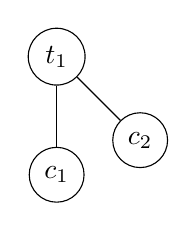
\begin{tikzpicture}[node distance={15mm}, main/.style = {draw, circle}] 
      \node[main] (1) {$t_1$}; 
      \node[main] (2) [below of=1] {$c_1$}; 
      \node[main] (3) [below right of=1] {$c_2$}; 

      \draw (1) -- (2); 
      \draw (1) -- (3); 
    \end{tikzpicture} 
    \caption{Denormalized graph repr.}
    \label{figure:denormalized-graph-representation}
  \end{minipage}
  \hfill
  \vspace{1em}
\end{figure}


Now measuring the distance between the graphs displayed in~\ref{figure:normalized-graph-representation} and~\ref{figure:denormalized-graph-representation}


% TODO: Finish this section on WWL graph kernels and distance calculation..

%is a set of id and distance tuples $\{(s_1, d_1), ..., (s_i,d_i)\}$
%where $s$ is the database schema name and $d$ is the distance to the
%\textit{current} schema. Thus a schema distance index has to be computed for each database schema
%\textsc{Natural} is running on.

%Thus.. $\mathcal{D}$
